\subsection{Цель выполнения лабораторной работы}\label{blockN.VariantM}
\textbf{Цель выполнения лабораторной работы }-- \GoalOfResearch

%-------------------------------------------------
\subsection{Задание}
Для цепи Маркова, заданной стохастической матрицей переходов: 
\begin{enumerate}
    \item нарисовать граф цепи; 
    \item проверить выполнение критерия эргодичности;
    \item рассчитать предельные вероятности;
    \item записать предельную матрицу переходов; 
    \item провести имитационное моделирование системы, соответствующей рассматриваемой цепи, для этого: 
    \begin{itemize}
        \item случайно выбрать начальное состояние; 
        \item случайно разыграть переход в новое состояние, учитывая распределение вероятностей перехода; 
        \item совершить 100 переходов; 
        \item повторить эксперимент 20 раз; 
        \item подсчитать число вхождений в каждое из состояний системы;
        \item  построить <<графики>> переключений состояний цепи (для наглядности соединяем дискретные точки); 
        \item составить таблицу для сравнения относительных частот наблюдений вхождения в каждое из состояний системы, указав исправленные оценки среднеквадратичных отклонений указанных относительных частот
    \end{itemize}
\end{enumerate}
%-------------------------------------------------
\newpage
\subsection{Решение}
Дана стохастическая матрица переходов $\mathbf{P}$:
$$\mathbf{P}=\begin{pmatrix}
0.17& 0.28& 0.17& 0.15& 0.23\\
0.23& 0.20& 0.18& 0.18& 0.21\\
0.22& 0.18& 0.25& 0.15& 0.20\\
0.26& 0.16& 0.20& 0.16& 0.22\\
0.19& 0.24& 0.21& 0.14& 0.22
\end{pmatrix}$$

На рисунке \ref{graph} представлен граф переходов, соответствующий матрице $\mathbf{P}$.
\begin{figure}[!h]
\centerline{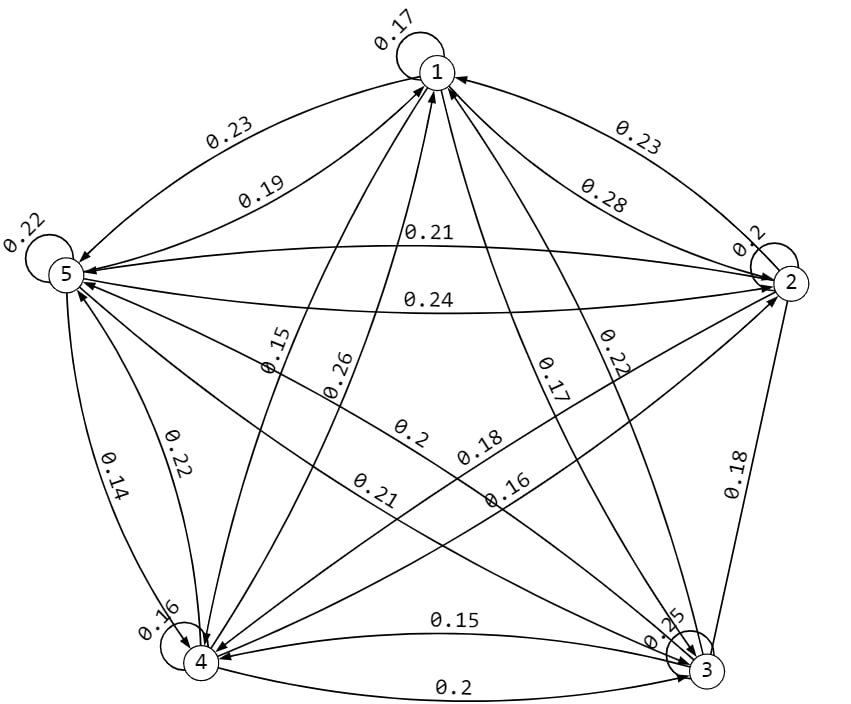
\includegraphics[scale = 1.1]{Images/graph.jpg}}
\caption{Граф переходов}
\label{graph}
\end{figure}

\subsubsection{Определение вектора предельных вероятностей, проверка выполнения условия эргодичности}


$$(\mathbf{P}^T-\mathbf{E})\times\overline{p}=\overline{0},$$
где $\overline{p}$--вектор предельных вероятностей

Однако, поскольку система является линейно зависимой в качестве последнего уравнения внесем условие $\sum\limits_{i=1}^5p_i=1$.

Была реализована функция, вычисляющая вектор предельных вероятностей  $\overline{p}$, формирующая предельную матрицу переходов, а также проверяющая критерий эргодичности.

\begin{lstlisting}[language=python, label=prog,caption={\textit{расчет вектора предельных вероятностей}}]
def marginal_probabilities(P):
    A = P.T - np.eye(len(states), dtype=float)
    A[-1] = np.full(len(states), 1)
    b = np.zeros(len(states))
    b[-1] = 1.
    p = np.linalg.solve(A, b)
    return p, [list(p) for _ in range(len(states))], list(p).count(0)!=len(p)
\end{lstlisting}

~\\

Таким образом, вектор вектор предельных вероятностей:
$$\overline{p}=(0.21134212\quad 0.21527835\quad 0.20159311\quad 0.15585764\quad 0.21592878)^T$$

Предельная матрица переходов:

$$\mathbf{P(n)}=\begin{pmatrix}
0.21134212 &0.21527835 &0.20159311 &0.15585764 &0.21592878\\
0.21134212 &0.21527835 &0.20159311 &0.15585764 &0.21592878\\
0.21134212 &0.21527835 &0.20159311 &0.15585764 &0.21592878\\
0.21134212 &0.21527835 &0.20159311 &0.15585764 &0.21592878\\
0.21134212 &0.21527835 &0.20159311 &0.15585764 &0.21592878
\end{pmatrix}$$

\underline{цепь эргодична}

~\\

\subsubsection{Имитационное моделирование}

 Была разработана функция, реализующая переходы, заданное число раз, возвращающая траекторию и словарь с количеством посещений для каждого состояния (ключи--состояния).

 \begin{lstlisting}[language=python, label=prog,caption={\textit{реализация марковского процесса}}]
def mark_iter(n, m, states):
    current_s = randrange(1,6)
    states_tr = [current_s]
    for _ in range(n-1):
        per_ver = m[current_s-1]
        next_s = np.random.choice(states, p=per_ver)
        current_s=next_s
        states_tr.append(current_s)
    return dict(sorted(dict(Counter(states_tr)).items())), states_tr
\end{lstlisting}

На рисунке \ref{iter} представлены «графики» переключений состояний цепи.

\begin{figure}[!h]
\centerline{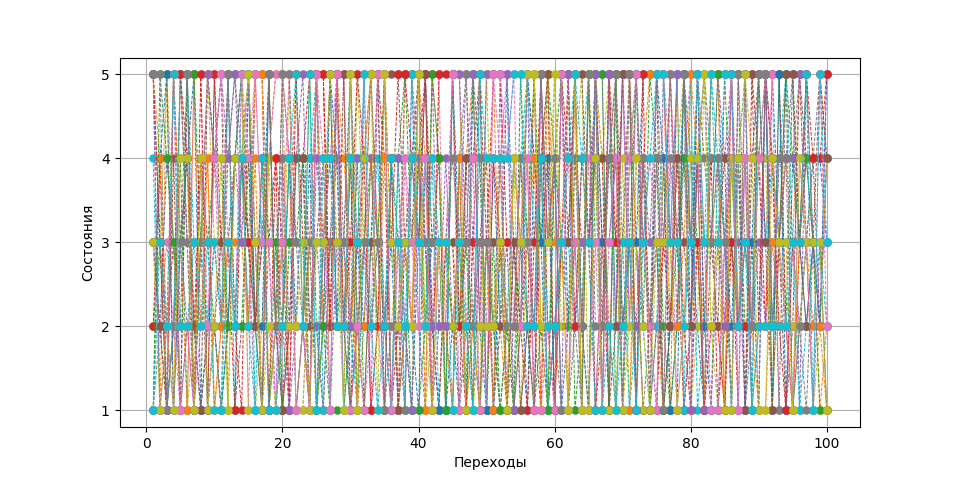
\includegraphics[scale = 1.]{Images/iter.png}}
\caption{Переключения состояния цепи}
\label{iter}
\end{figure}



%-------------------------------------------------
%-------------------------------------------------

%-------------------------------------------------
\subsection{Вывод}
В ходе выполнения лабораторной работы был реализован МКЭ для различных функций форм, а также найдено количество линейных КЭ обеспечивающих точность 20ти кубических КЭ.

% --------------------------------------
% Атрибуты задачи
\labattributes{}{}{}{}{студент группы \EduGroup, \Author}{\Year, \Semestr}
%--------------

